\section{O OpenServer}
    
    Para desenvolver o OpenServer foi aproveitada a estrutura padrão do sistema fornecida pela empresa fabricante, como detalhado na Figura~\ref{conexoes-padrao}, onde: (1) é a conexão elétrica entre Controladora e Manipulador Robótico; (2) representa a conexão \textit{PowerLink} entre \textit{LPC} e controladora; (3) é a conexão entre roteador e controladora; e (4) conexão entre roteador e o \textit{LPC}.

    \begin{figure}[ht]
        \centering
        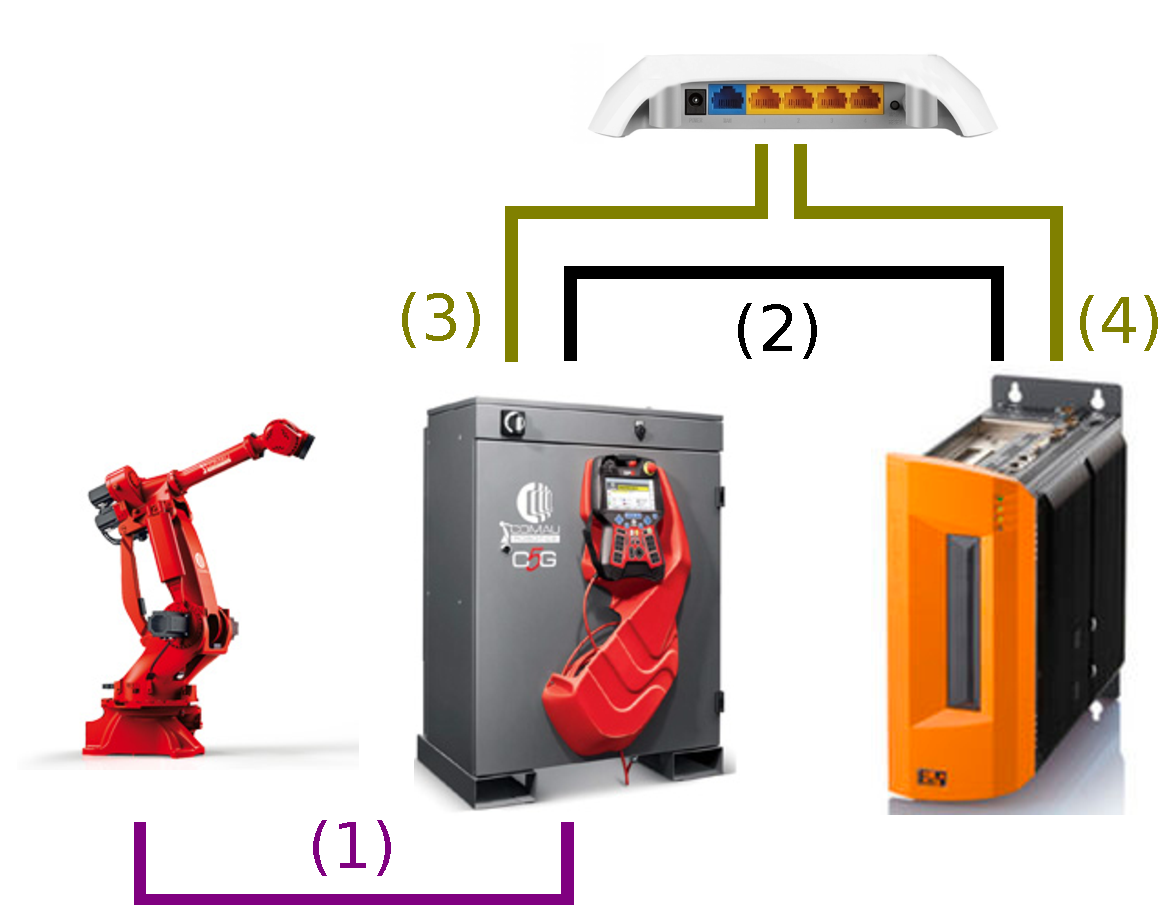
\includegraphics[width=\columnwidth]{imagens/Conexoes/conexoes-padrao.eps}
        \small 
        \centering 
        \caption{Estrutura padrão do sistema C5G Open}
        
        \label{conexoes-padrao}
    \end{figure}
      
    O OpenServer é um software do tipo servidor que permite o desenvolvimento de programas clientes que recebam por ele os dados sensoriais vindos da controladora do robô e envie através dele os comandos de movimentação para a mesma. No entanto, essa comunicação passará a ser feita usando uma rede \textit{Ethernet} convencional, através do uso do protocolo TCP/IP. Isso permite que o programa cliente possa ser programado na linguagem de programação de preferência do usuário, rodando em uma arquitetura e sistema operacional disponíveis.
    
    Para isso, o OpenServer foi programado dentro das limitações da plataforma, ou seja, na linguagem C++ usando a biblioteca \textit{eORL} do fabricante do robô, usando a rede \textit{PowerLink} para fazer a comunicação com a controladora do robô e sendo compilado para o sistema operacional baseado em Linux com arquitetura x86. Além disso, ele usa bibliotecas padrão em C++ disponíveis para o sistema operacional \textit{Linux Mint} para realizar a comunicação via rede TCP/IP. A estrutura desenvolvida para execução do OpenServer passa então a ser conforme mostra a Figura~\ref{conexoes-openserver}, onde: (5) representa a conexão entre o roteador e o dispositivo externo, a qual, pode ser feita através de cabeamento ou conexão sem fio; e (6) é a conexão entre roteador e rede institucional.
    
    \begin{figure}[ht]
        \centering
        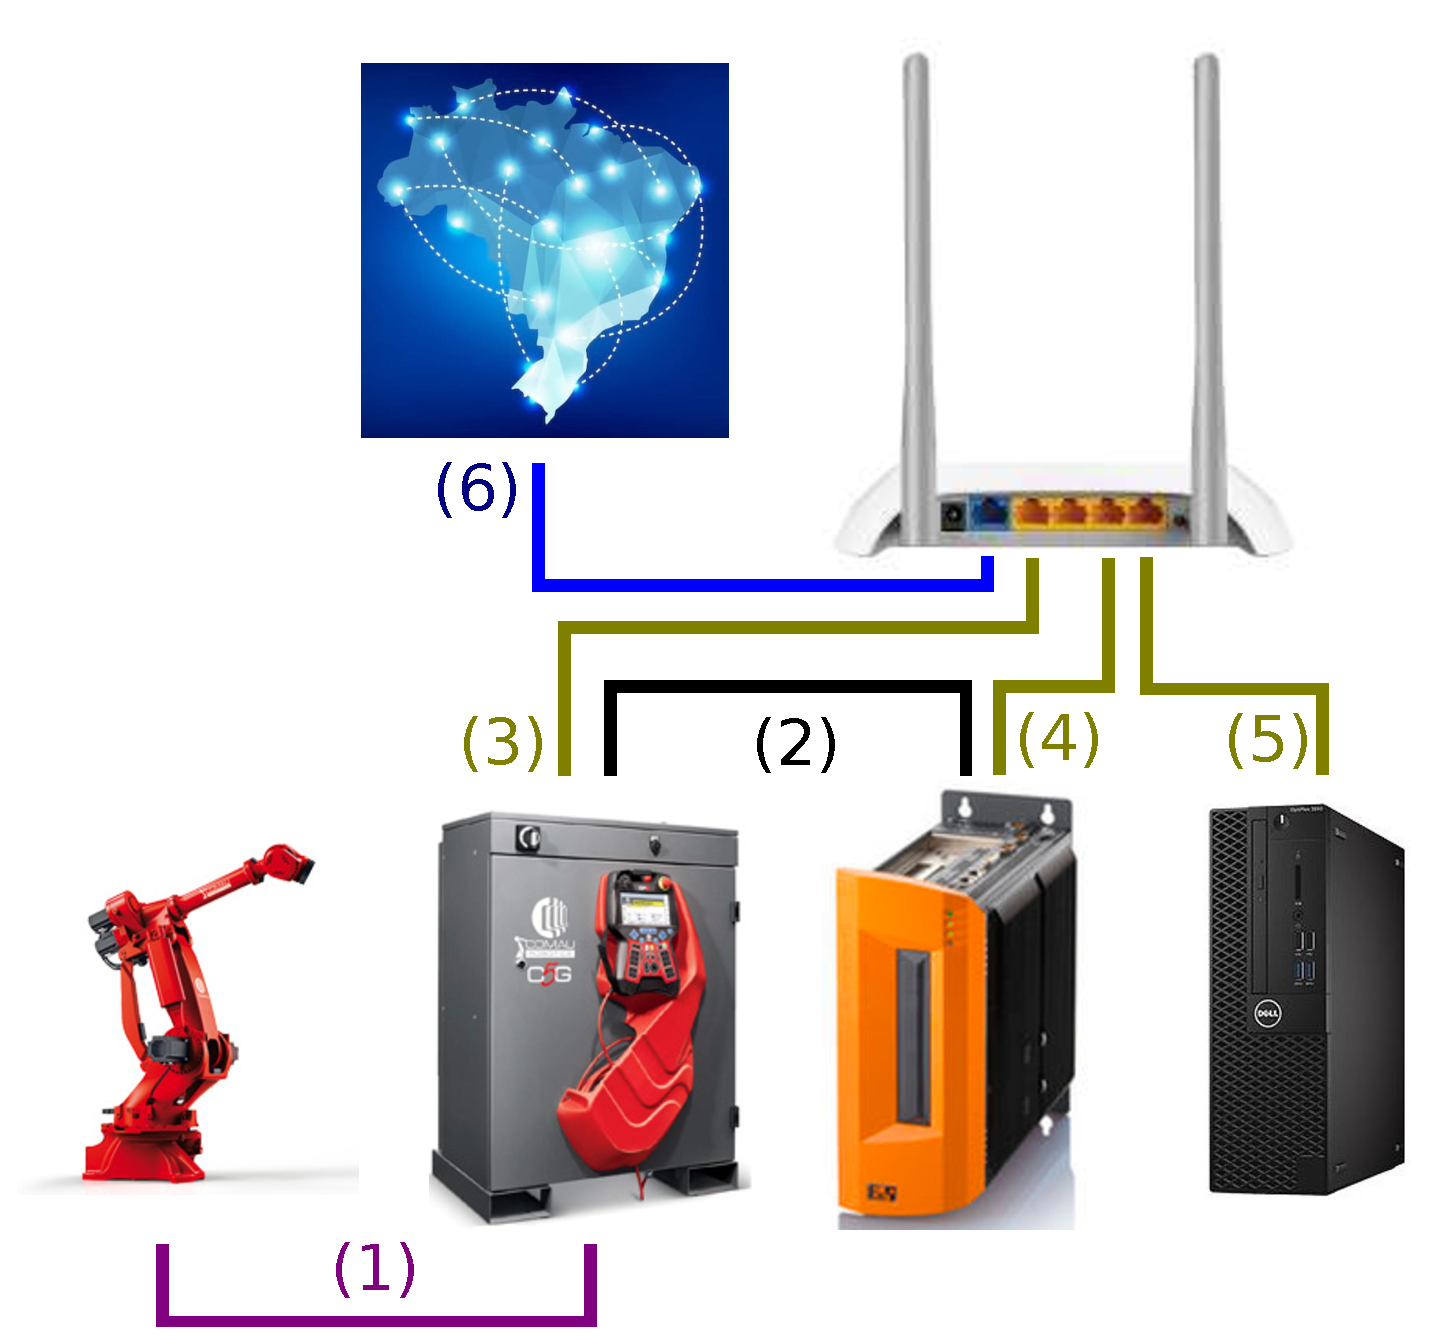
\includegraphics[width=\columnwidth]{imagens/Conexoes/conexoes-openserver.eps}
        \small 
        \centering 
        \caption{Estrutura desenvolvida para execução do OpenServer}
        
        \label{conexoes-openserver}
    \end{figure}
    
    
    A rede institucional do CEFET-MG oferece acesso à internet. No entanto, as portas do roteador são bloqueadas para acesso externo. Dessa forma, é criada uma rede interna segura onde os softwares são executados. Por esta razão, não foram implementadas soluções de criptografia de dados, bem como de autenticação. Isso ocorreu também pelo motivo de ser um ambiente acadêmico, controlado e sem trafego de dados sensíveis. A estrutura real do sistema pode ser visto na Figura~\ref{lab1}.
    
    \begin{figure}[ht]
        \centering
        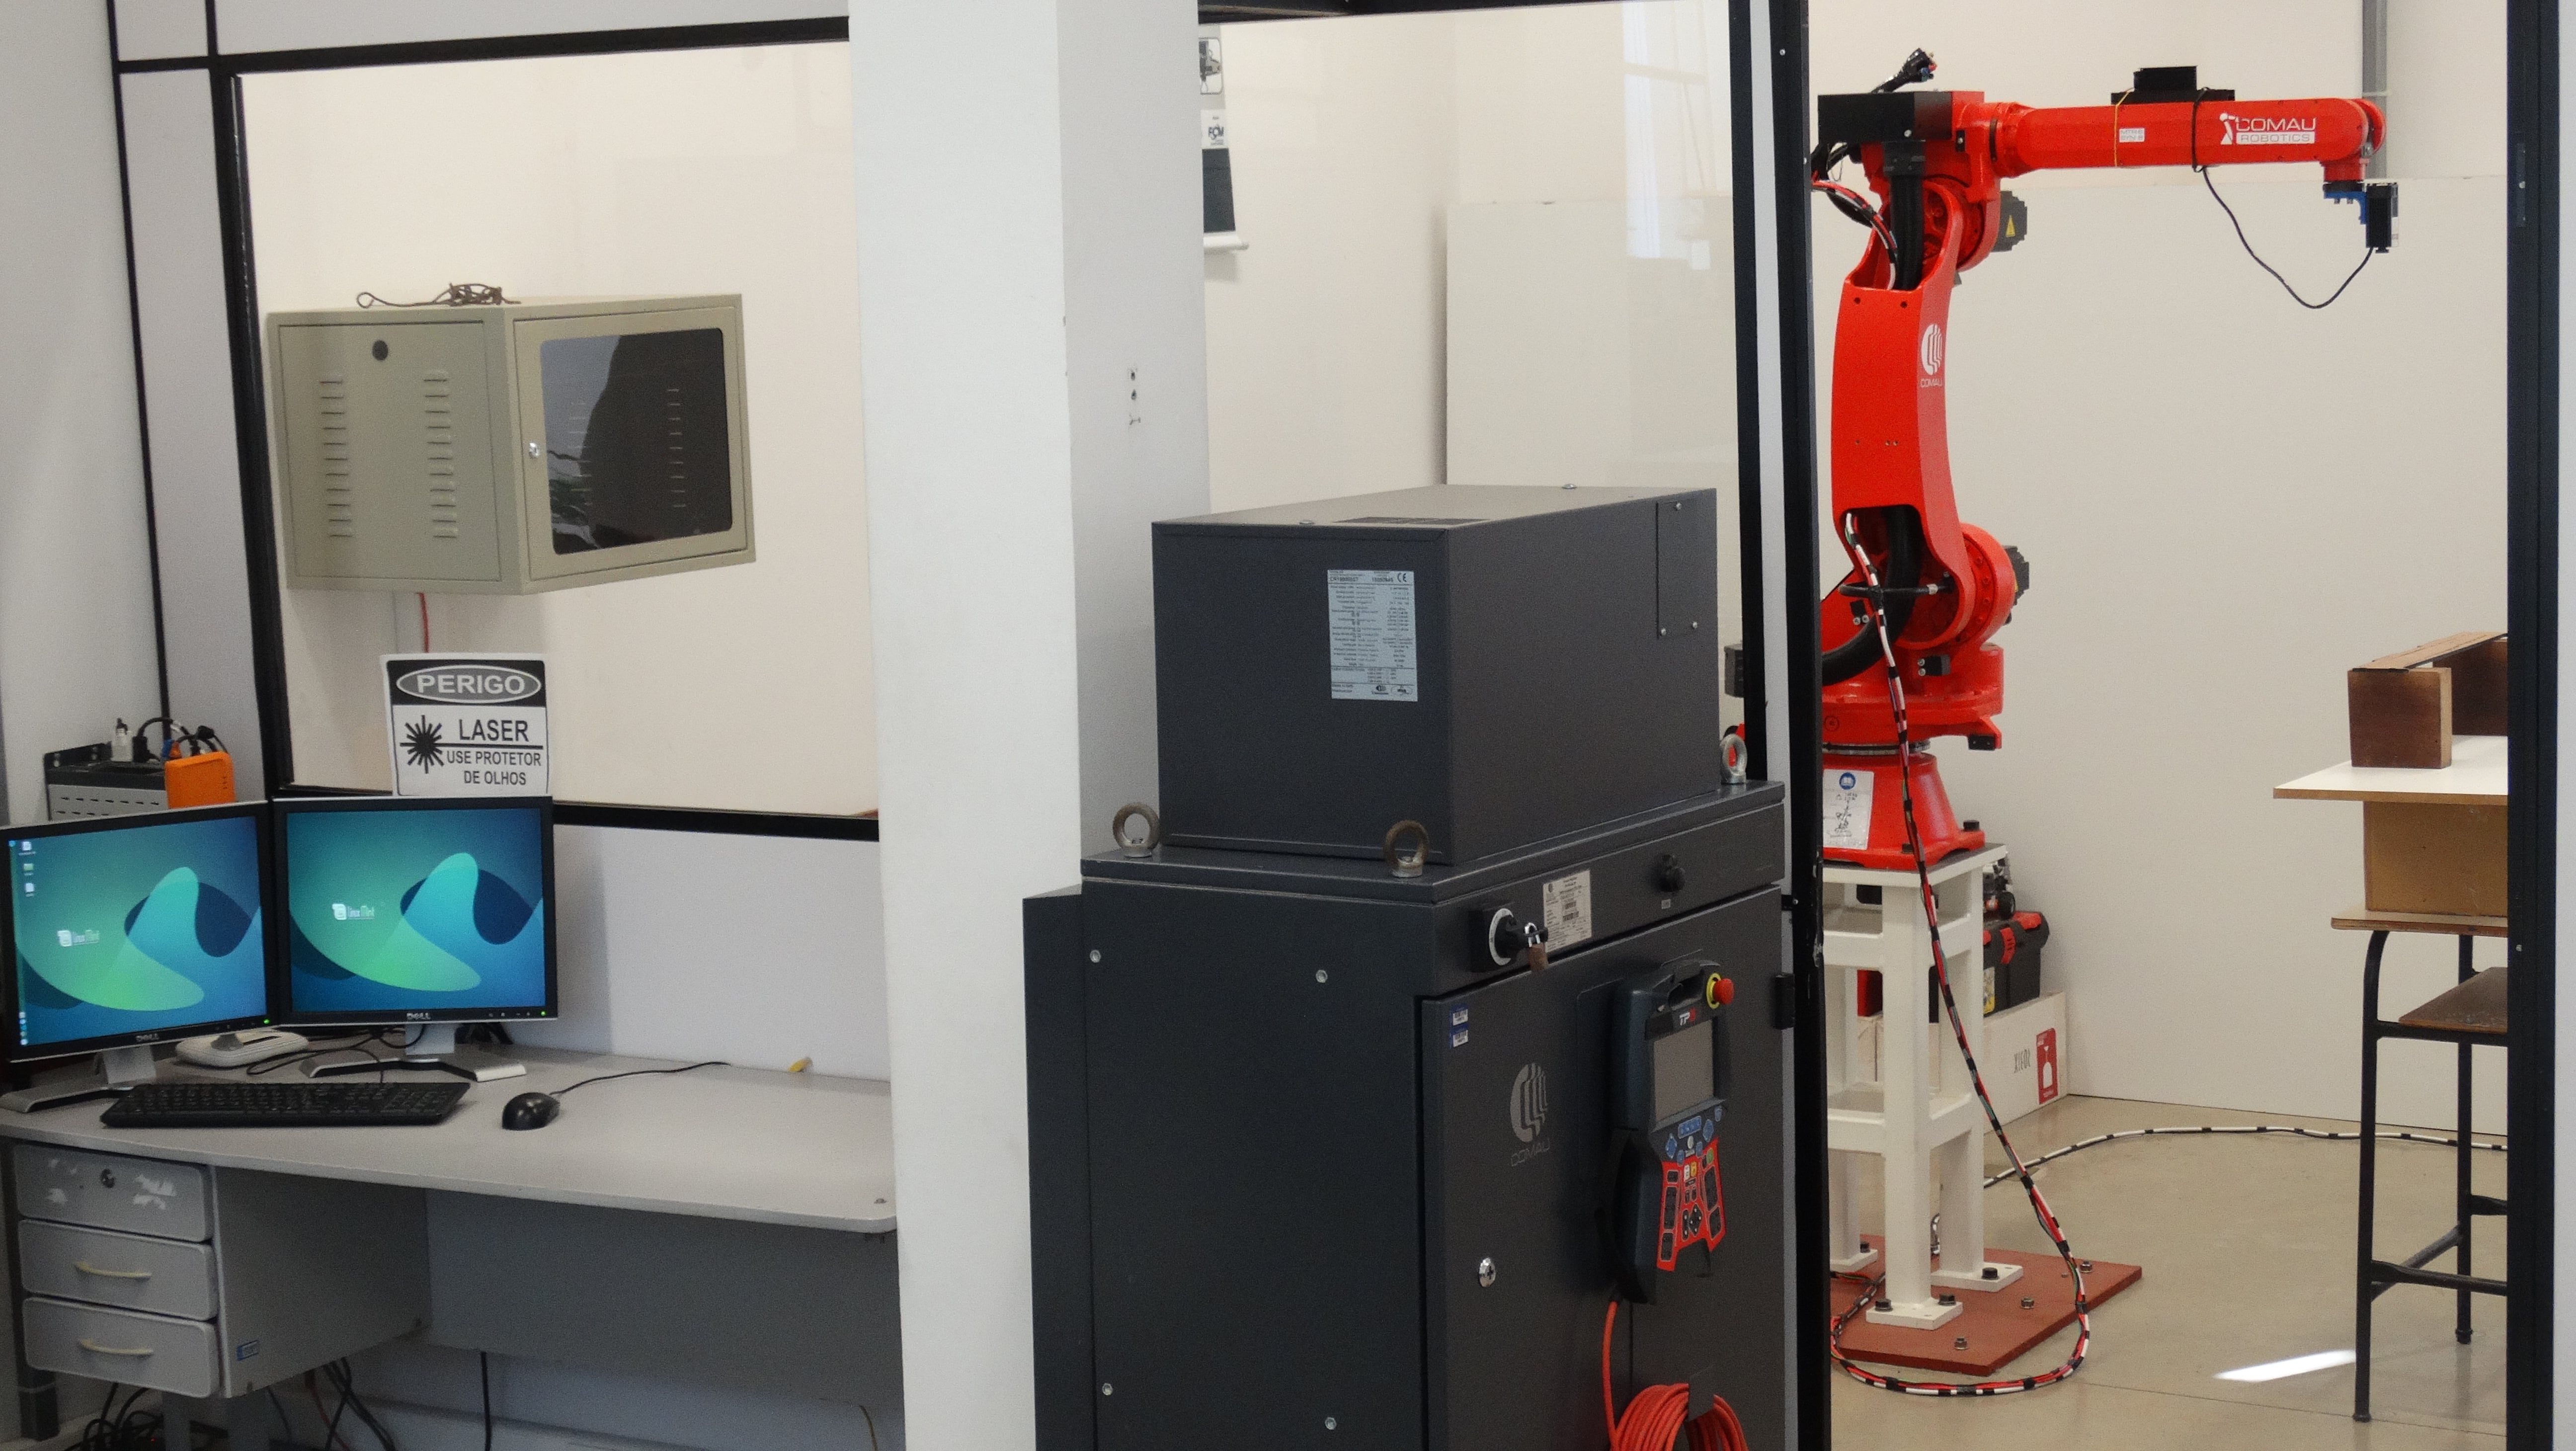
\includegraphics[width=\columnwidth]{imagens/Fotos/estrutura-lab-1.JPG}
        \small 
        \centering 
        \caption{Estrutura do laboratório onde será executado o OpenServer}
        \label{lab1}
    \end{figure}
    
    Estão disponíveis dois computadores para a execução de programas cliente, que podem ser vistos na Figura~\ref{lab2}, conectados à rede interna.
    
    \begin{figure}[ht]
        \centering
        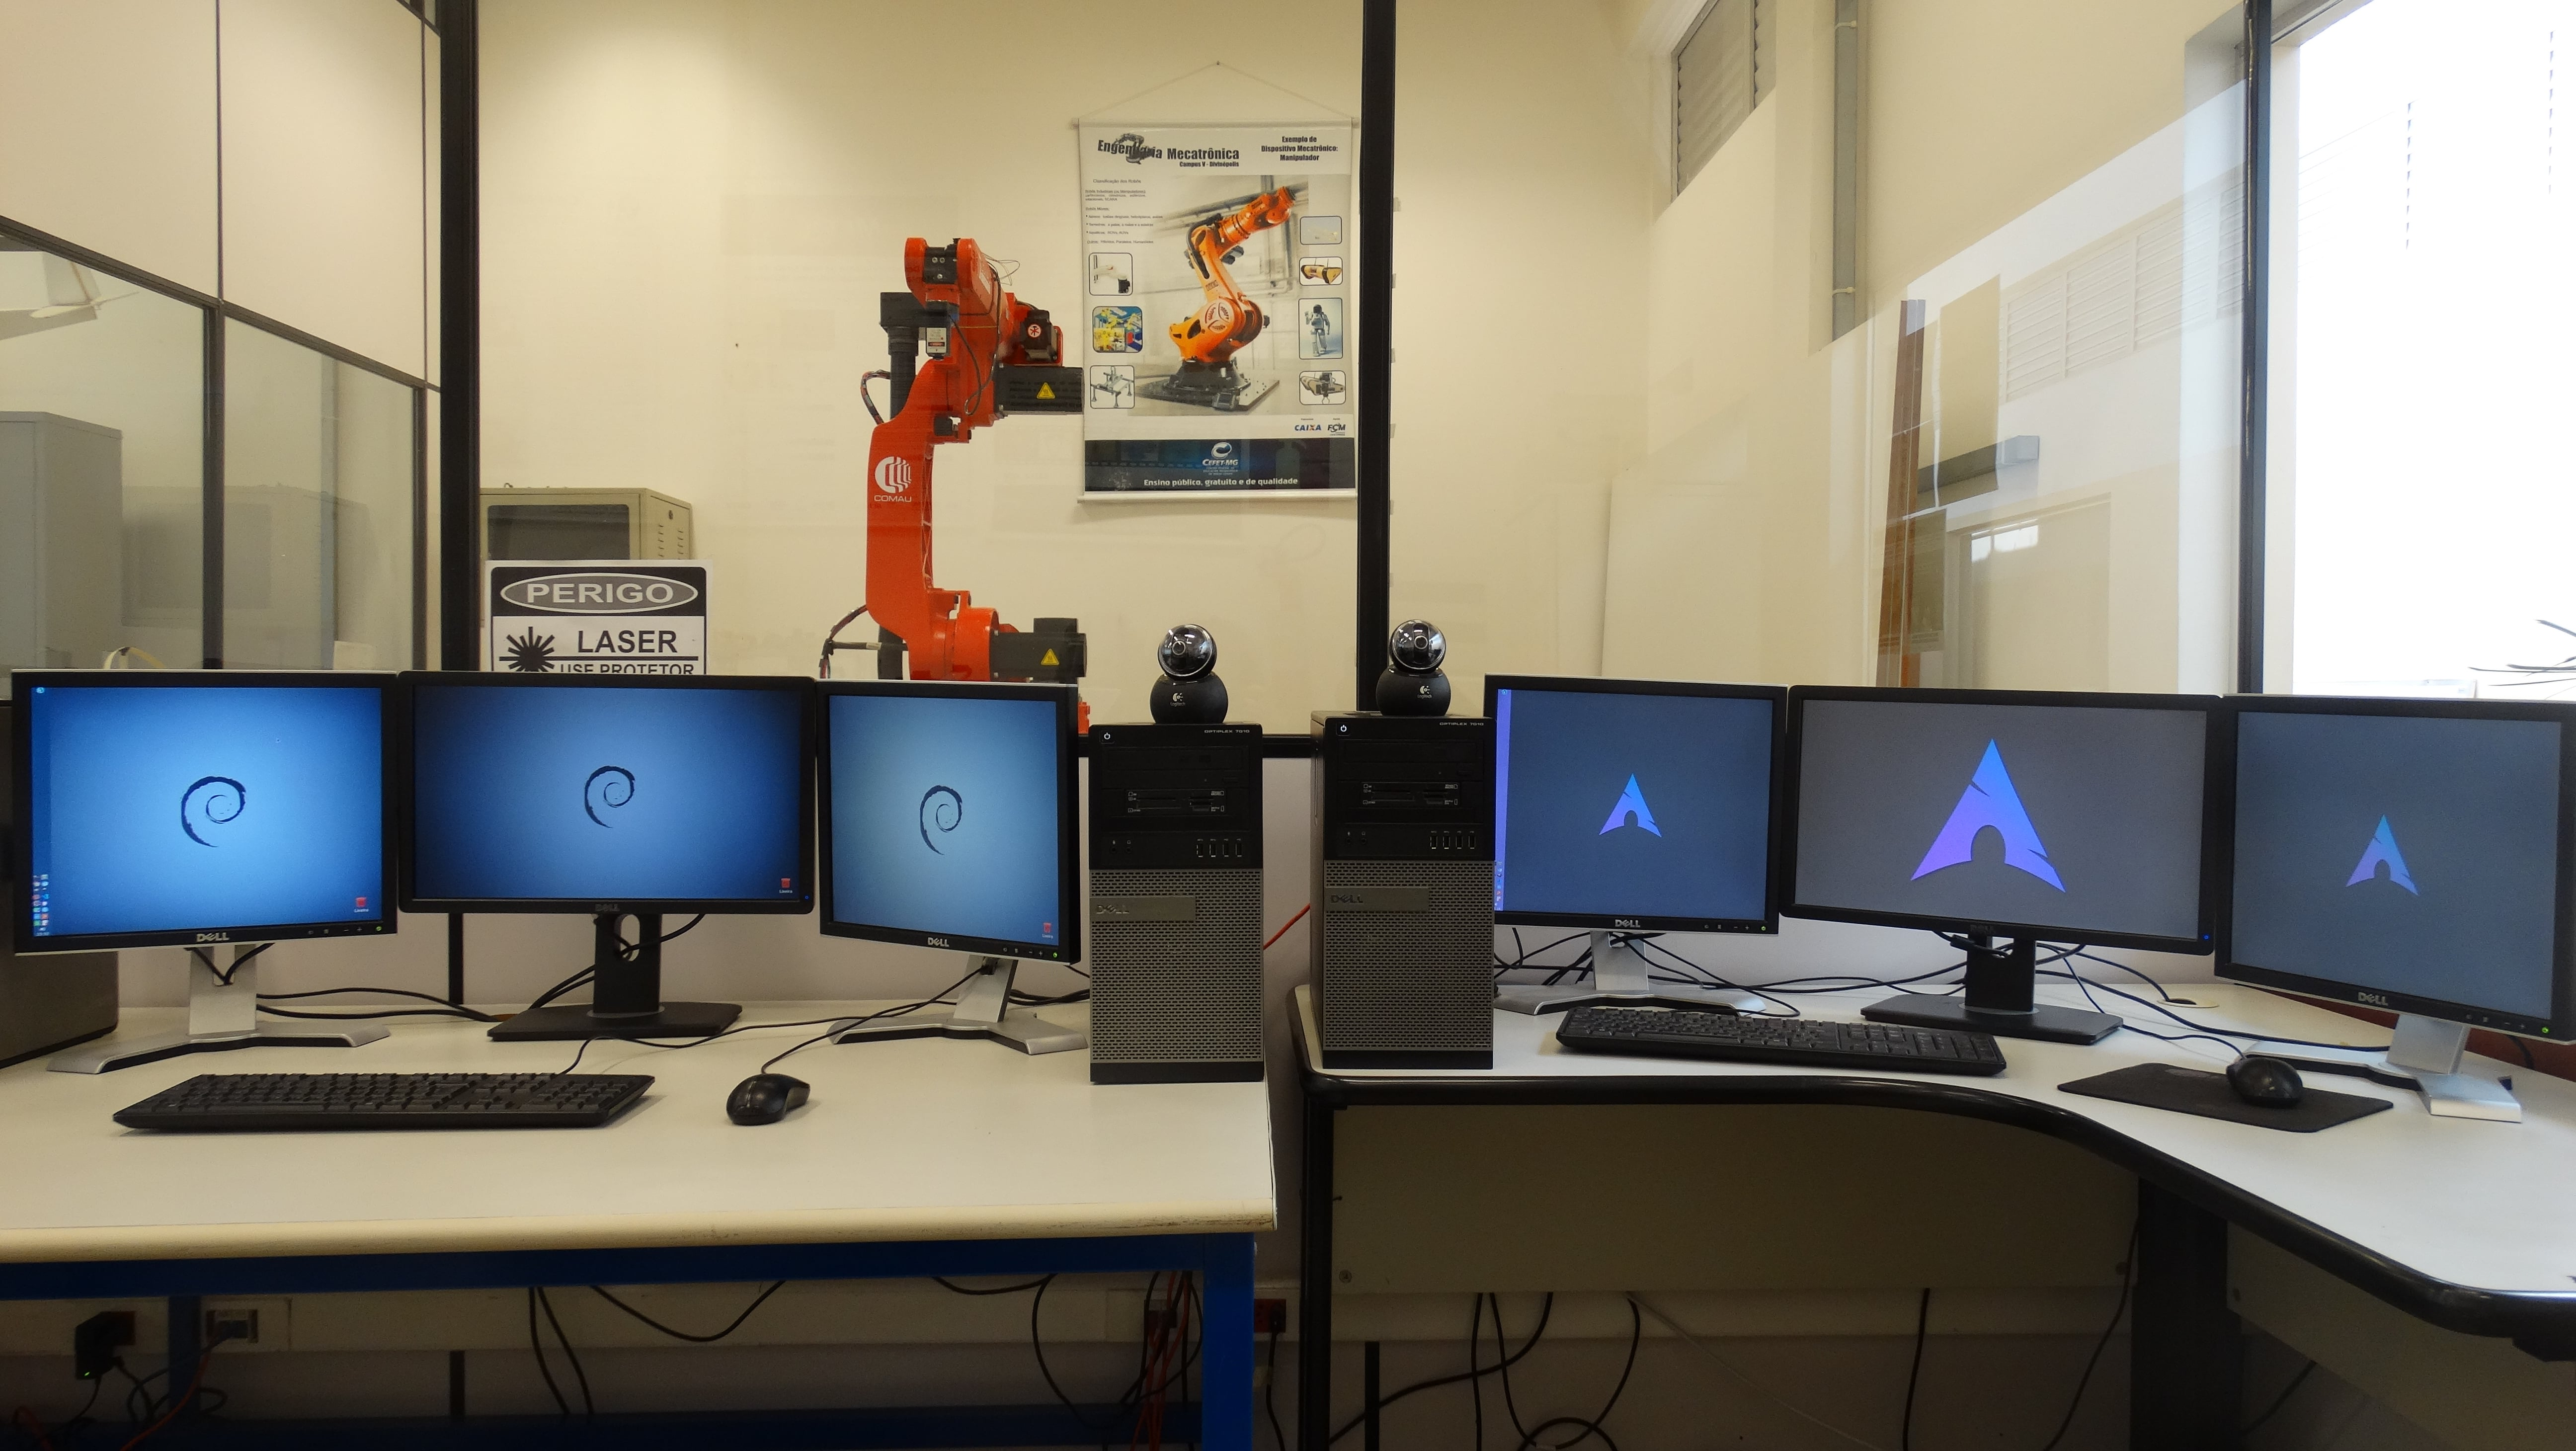
\includegraphics[width=\columnwidth]{imagens/Fotos/estrutura-lab-2.JPG}
        \small 
        \centering 
        \caption{Estrutura do laboratório onde será executado o OpenServer}
        \label{lab2}
    \end{figure}
        
    Para utilizar o sistema \textit{Open} é crucial a instalação da biblioteca \textit{eORL} no \textit{LPC} na mesma versão da \textit{eORL} da controladora~\citep{Open:Manual}. No caso, essa biblioteca já estava instalada no LPC, sendo necessária apenas a atualização dela para a última versão estável. Além disso, quando se desejar usar o sistema Open, é necessário habilitar o modo Open nos eixos desejados dentro do programa \textit{Crcopen}, conforme indicado na Figura~\ref{habilitar-open}.
    
    \begin{figure}[ht]
        \centering
        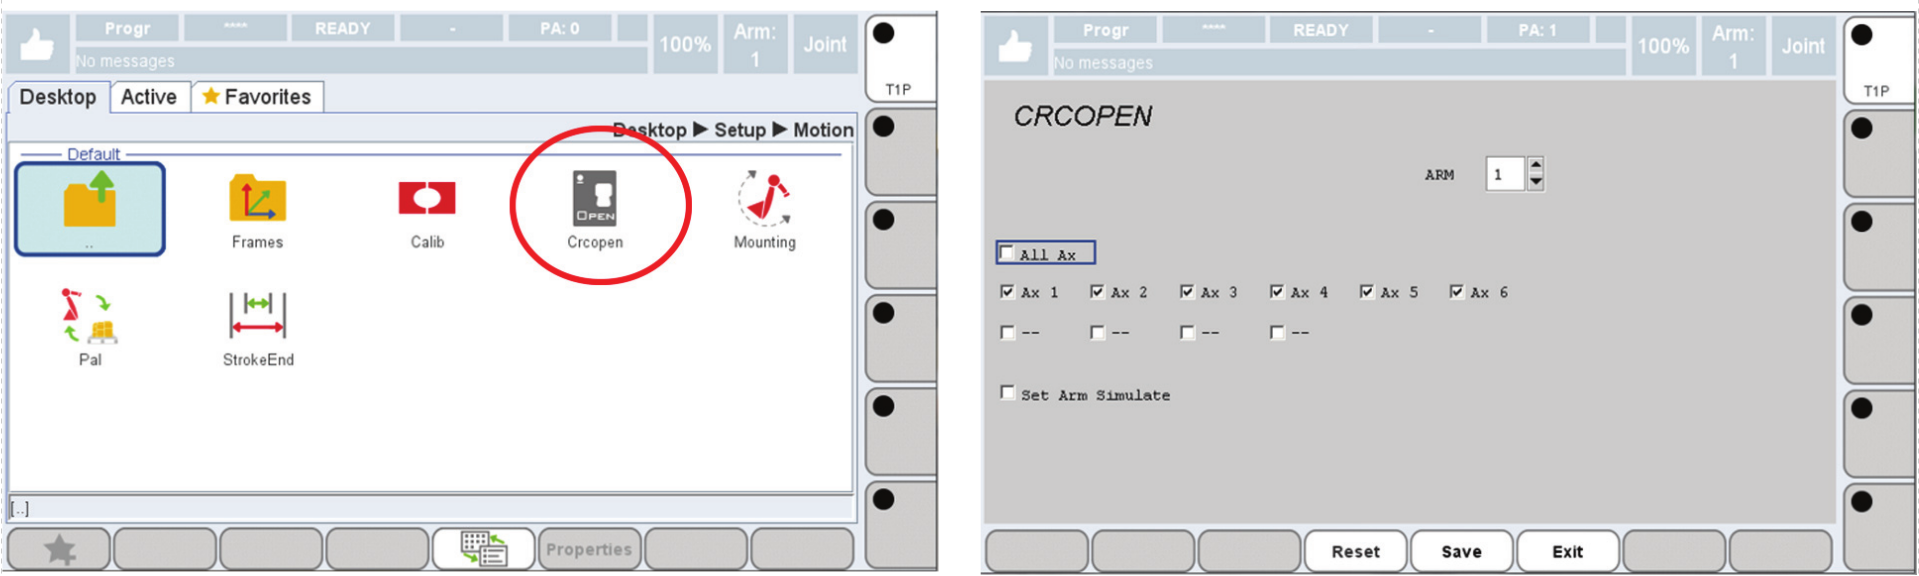
\includegraphics[width=\columnwidth]{imagens/Softwares/habilitar-open.png}
        \small 
        \centering 
        \caption{Procedimento para habilitar o modo Open dos eixos do robô~\citep{Open:Manual}}
        \label{habilitar-open}
    \end{figure}
    
    O desenvolvimento deste software torna mais segura a utilização do sistema Open em um ambiente de ensino e pesquisa, pois, o único software que precisará ser executado no \textit{LPC} passa a ser o \textit{OpenSever} em sua versão estável. Já no dispositivo externo serão executados os softwares experimentais, em desenvolvimento, os quais podem travar durante a execução. Quando isso acontece, o \textit{OpenSever} continua sendo executado no \textit{LPC} e comunicando com a controladora do robô, enviando a última referência armazenada. Dessa forma, o risco de se interromper bruscamente a comunicação com a controladora é evitado.
    
    Além disso, o \textit{OpenSever} expõe apenas um subconjunto das funcionalidades e configurações da \textit{eORL}, simplificando a utilização e reduzindo a quantidade de erros possíveis.
    
    \subsection{Funcionamento}
    
        Foi implementado um modo \textit{DEBUG}, a ser ativado antes do processo de compilação que imprime no terminal qual função foi executada, o comando vindo do programa cliente e a resposta enviada, conforme pode ser visto nas Figuras~\ref{openserver-wait}, \ref{openserver-ok}~e~\ref{openserver-send}. Quando o modo \textit{DEBUG} não está ativado apenas a biblioteca \textit{eORL} imprime textos no terminal, por exemplo, a tela de boas vindas, mensagens de erro, entre outros.
        
        Quando o software é executado, ele tenta se conectar com a controladora usando a biblioteca \textit{eORL} através da rede \textit{Powerlink}. Quando a conexão é bem sucedida o software entra em modo \textit{Listen}, ou seja, fica esperando um cliente se conectar ao \textit{soket} através da rede TCP/IP via \textit{Ethernet}, conforme pode ser visto na Figura~\ref{openserver-wait}.
        
        \begin{figure}[ht]
            \centering
            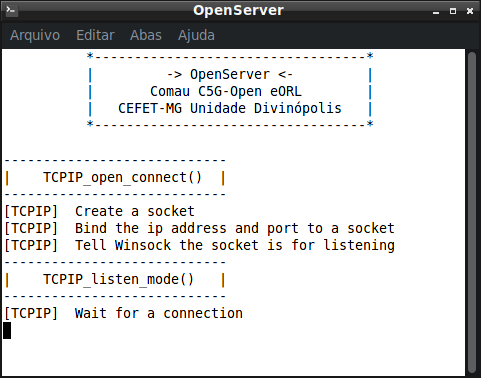
\includegraphics[width=\columnwidth]{imagens/Softwares/openserver-wait_.png}
            \small 
            \centering 
            \caption{OpenServer esperando a conexão de um \textit{software} cliente}
            \label{openserver-wait}
        \end{figure}
        
        Quando um cliente se conecta ao servidor é realizada uma troca de pacotes para verificar a integridade da conexão. Caso essa verificação seja bem sucedida o servidor fica esperando o recebimento de instruções do cliente, conforme pode ser visto na Figura~\ref{openserver-ok}. O servidor só atua mediante os comandos do cliente.
        
        \begin{figure}[ht]
            \centering
            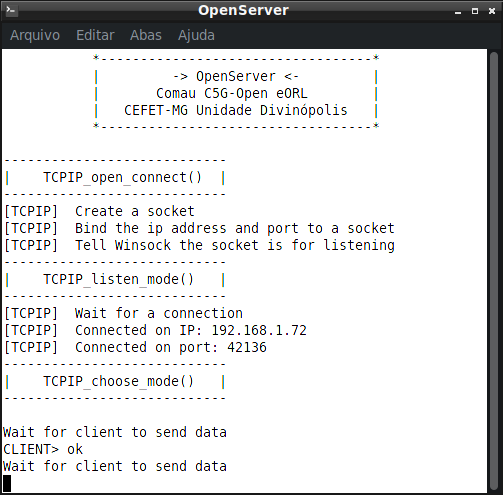
\includegraphics[width=\columnwidth]{imagens/Softwares/openserver-ok_.png}
            \small 
            \centering 
            \caption{OpenServer esperando a instrução do \textit{software} cliente conectado}
            \label{openserver-ok}
        \end{figure}
        
        O primeiro caractere recebido pelo servidor informa qual procedimento ele deve seguir. No caso, a instrução `p' é atualmente a instrução padrão. Ela está configurada para os valores de referência das juntas do robô (truncado em 5 casas decimais, mas, sem uso da vírgula para representar as casas decimais) virem concatenados na forma de \textit{strings} logo após tal instrução, como pode ser visto na Figura~\ref{openserver-send}. Ao receber essa instrução, imediatamente o servidor atualiza as variáveis de referência das juntas do robô na biblioteca \textit{eORL}, as quais são enviadas para a controladora. Em seguida, também na forma concatenada sem uso de virgula, o servidor envia a resposta ao programa cliente com a leitura mais recente dos sensores das juntas do robô armazenada na memória do servidor, as quais, foram recebidas da controladora aberta.
        %Logo em seguida, a controladora envia a resposta ao programa cliente com os valores atuais dos sensores das juntas do robô, também na forma concatenada sem uso de virgula. 
        
        \begin{figure}[ht]
            \centering
            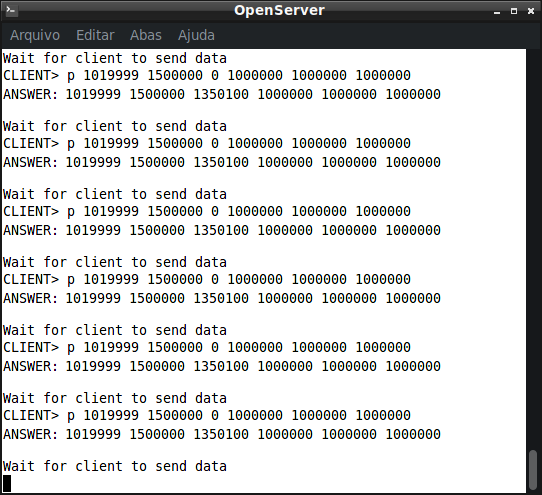
\includegraphics[width=\columnwidth]{imagens/Softwares/openserver-send_.png}
            \small 
            \centering 
            \caption{OpenServer executando a instrução do \textit{software} cliente e respondendo com a leitura dos sensores}
            \label{openserver-send}
        \end{figure}
        
        Esta forma de transmitir os dados (\textit{strings} concatenadas) foi desenvolvida com a intenção de ser uma construção simples de ser implementada em outras linguagens de programação.

        Como as taxas de transmissão de dados podem não ser necessariamente as mesmas, foi implementado um algoritmo interno que resolve esse problema de falta de sincronia. Por exemplo, a taxa de comunicação da \textit{eORL} com a controladora varia de uma taxa de $0,4\,\mathrm{ms}$ a $16\,\mathrm{ms}$; e a taxa de comunicação entre o programa servidor e o programa cliente não tem uma faixa definida. Assim, o desenvolvedor do programa cliente tem a liberdade de programar a taxa que for mais conveniente (dentro dos limites práticos da rede) e, inclusive, enviar os comandos de movimentação de forma não constante.
        